\chapter{Contextualización}
\label{cap:Contextualizacion}

\definecolor{lightergray}{RGB}{247,247,247}
\definecolor{darkgreen}{RGB}{36,135,20}
\definecolor{green_comment}{RGB}{0,128,0}
\definecolor{redcell}{RGB}{238,176,176}
\definecolor{greencell}{RGB}{217,234,211}


En este capítulo se presenta una breve descripción de los algoritmos de Inteligencia Artificial que se van a profundizar a lo largo del proyecto. Así como los usos y características. 

El objetivo de este capítulo es explicar rápidamente los algoritmos, y facilitar la lectura de los capítulos posteriores. Que desarrollen las mejoras realizadas y resultados obtenidos.



\section{MPI}
Message Passing Interface \cite{barker2015message}  (MPI)  es un estándar para una biblioteca de paso de mensajes, diseñado para funcionar en una amplia variedad de arquitecturas informáticas paralelas. Permite la comunicación entre procesos, mandando y recibiendo mensajes de todo tipo. Comúnmente usado en informática de alto rendimiento \cite{stone1990high} (HPC) y entornos informáticos paralelos, para desarrollar aplicaciones paralelas escalables y eficientes.

Al crear el entorno MPI en una aplicación se ejecutan en paralelo varios procesos, cada uno con su correspondiente id. El primer proceso (id=0) es llamado Master, se encarga de distribuir los mensajes entre los demás procesos, workers, para que haya una comunicación eficiente y paralelizar los programas. Figura \ref{fig:comunicacion_mw}.

Esta técnica para paralelizar utiliza memoria distribuida, es decir, cada proceso tiene su propia memoria local. No tienen que preocuparse por los problemas de la memoria compartida, como la sincronización para el acceso de variables compartidas, condiciones de carrera o deadlocks. Asimismo la memoria compartida no es fácilmente escalable a un gran número de procesadores \cite{barker2015message} .


\textbf{Single Program Multiple Data (SPMD)}. Un programa ejecutado en paralelo. Este mismo se copia en todos los nodos. Figura \ref{fig:ejecucion_mpi}.

La comunicación se lleva a cabo con funciones punto a punto, un proceso emisor y otro receptor. Estos mensajes pueden ser:
Síncronos: al ejecutar la función recv() el proceso receptor se queda bloqueado.
Asíncrono: el receptor no se bloquea, por lo que puede adelantar código mientras espera a recibir el mensaje.
Broadcast:un mensaje se envía a todos los procesos ejecutados. Los emisores tienen que llamar a la misma función para recibir el mensaje.




\begin{figure}[!h]
\lstset{language=python, 
	language=python,
	breaklines=true,
	basicstyle=\footnotesize\ttfamily,
	backgroundcolor=\color{lightergray},
	keywordstyle=\color{blue}, % Keywords will be blue
	commentstyle=\color{green!60!black}, % Comments will be green
	stringstyle=\color{purple}, % Strings will be purple
	numbers=left, % Line numbers will appear on the left
	numberstyle=\tiny\color{gray}, % Line numbers will be small and gray
	frame=single,}
		
\begin{lstlisting}[frame=single]
from mpi4py import MPI #Al importar la biblioteca en Python se genera el entorno.

comm=MPI.COMM_WORLD     	# Comunicador
status = MPI.Status()   		# Status
myrank=comm.Get_rank() 	# id de cada proceso
numProc=comm.Get_size() 	# Numero de procesadores
if myrank==0:           # Master
# TODO
else:                   # Workers
# TODO	
\end{lstlisting}
\caption{Esquema básico para ejecutar un programa MPI en Python}
\label{fig:esquea_mpi}
\end{figure}


\begin{figure}[!h]
	\centering
	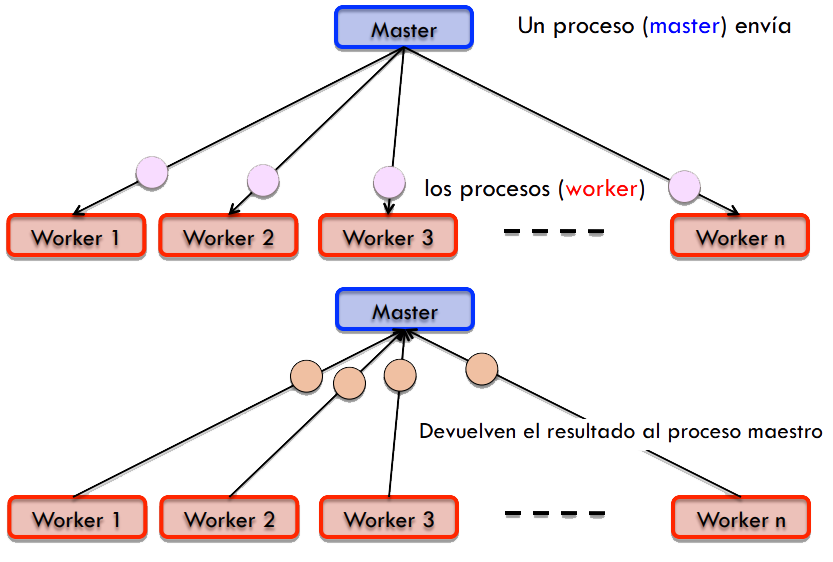
\includegraphics[width=0.6\textwidth]{images/chapter_2/mpi_1}
	\caption{Comunicación Master-Worker}
	\label{fig:comunicacion_mw}
\end{figure}

\newpage

\begin{figure}[!h]
	\centering
	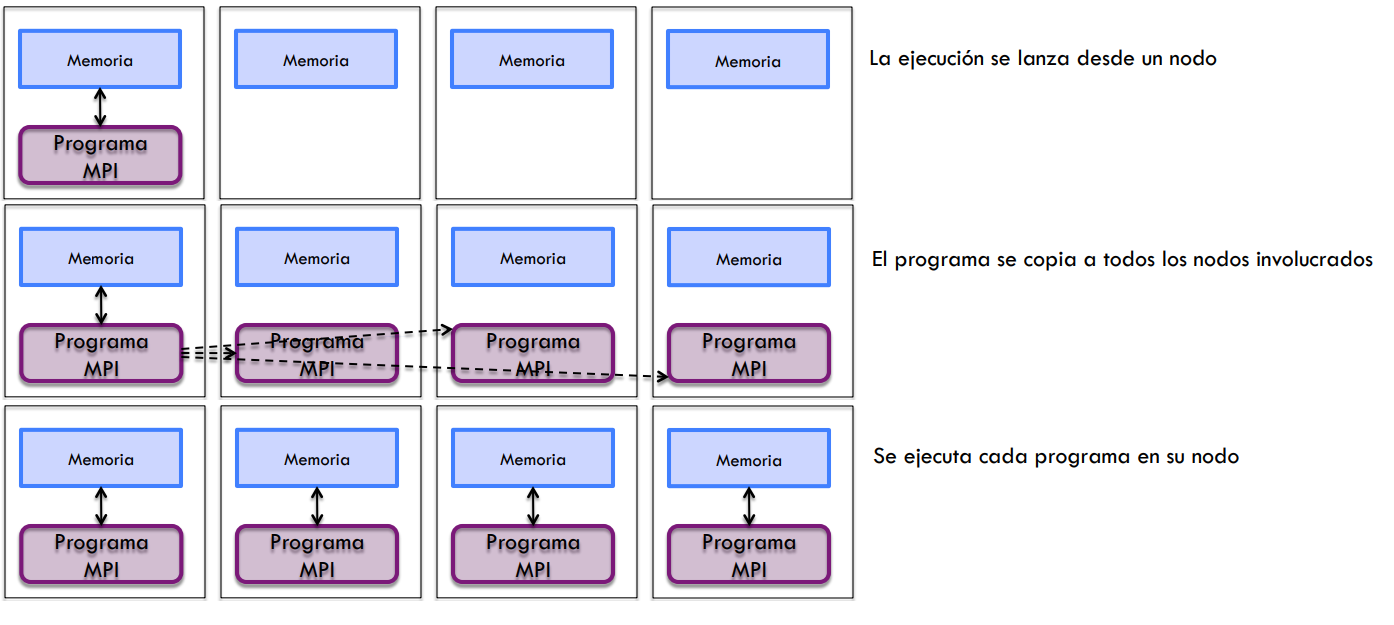
\includegraphics[width=0.8\textwidth]{images/chapter_2/mpi_2}
	\caption{Ejecución MPI}
	\label{fig:ejecucion_mpi}
\end{figure}


%\newpage

\section{Aprendizaje por Refuerzo}

Reinforcement Learning (RL), en español Aprendizaje por Refuerzo. Es un tipo de aprendizaje automático donde el agente aprende en base a las decisiones tomadas al interactuar con el entorno. El agente aprende a llegar a una meta o maximizar un cúmulo de recompensas obtenidas al realizar un determinado número de acciones consecutivas, y observar las posibles recompensas al realizar cada acción en los estados del entorno.

El agente aprende a con prueba y error, explorando las diferentes acciones y aprendiendo cuáles conducen a mejores resultados. No requiere entradas etiquetadas como en el aprendizaje supervisado, aprende con una serie de feedbacks (recompensas o castigos).

\begin{flushleft}
	Los componentes esenciales del algoritmo son los siguientes:
\end{flushleft}
\begin{itemize}
	\item Agente que interactúa con el entorno y aprende de él. 
	\item El entorno, con el cual el agente interactúa. Responde a las acciones tomadas por el agente y provee el feedback al agente.
	\item El conjunto de acciones o decisiones que el agente puede realizar.
	\item Estados. Situaciones de configuraciones en el entorno.
	\item Recompensas. Se suele representar como una matriz R(S,A), estados-acción. Almacena el feedback del entorno al realizar una acción en un estado.
	\item Q-Table Q(S,A). Guarda los valores-Q de las acciones en los estados.
	\item Condición de finalización. Puede ser desde encontrar la función-Q óptima, hasta realizar un número de épocas (Ejecución por el entorno, hasta finalizar una partida)
\end{itemize}


\noindent \textbf{Algoritmo Q-Learning:} Mezcla entre programación dinámica y Monte Carlo \cite{wang2012monte}.

Es el más básico de entre los algoritmos de aprendizaje por refuerzo. Se usa para encontrar la mejor política de selección de acciones para un proceso de Decisión de Markov Determinado (MDP en inglés) \cite{garcia2013markov}. 

El procedimiento se realiza actualizando iterativamente las estimaciones de calidad de realizar dicha acción en el estado actual, conocido como valor-Q. Este valor representa el feedback que recibirá el agente al realizar la acción desde un estado. Se usa la siguiente fórmula para actualizar los valores.

El agente toma las decisiones de ejecutar una acción dependiendo del hiper parámetro $\epsilon$  con valores entre [0,1]. Con un número aleatorio (en el mismo intervalo) calcula la probabilidad de ejecutar la mejor acción aprendida hasta el momento, o una acción aleatoria entre las disponibles. Si el valor es alto, casi siempre se ejecutará la “mejor” y es posible que no aprenda otras formas de alcanzar el objetivo.



\begin{flushleft}
	\begin{mdframed}[roundcorner=5pt]
		\[
		Q(S,A) = (1-\alpha) \cdot Q(S,A) + \alpha \cdot \left(R(S,A) + \gamma \cdot \max_{i} Q(S',A_i)\right)
		\]
		\begin{tcolorbox}[boxrule=0.5pt, fontupper=\small]
			\scriptsize
			Q(S,A) ← Es el valor-Q de ejecutar la acción A en el estado S.\\
			R(S,A) ← Es la recompensa obtenida al ejecutar la acción A en el estado S.\\
			$\alpha$ ← Tasa de aprendizaje. Controla cuánta importancia le da a la nueva información frente a la antigua.\\
			$\gamma$ ← Factor de descuento. Determina la importancia de futuras recompensas comparadas con las recompensas inmediatas.\\
			maxi(Q(S’,Ai)): Es el valor máximo obtenible de realizar las posibles acciones en el estado siguiente.
			
			
		\end{tcolorbox}
		
	\end{mdframed}
\end{flushleft}

%\newpage

Este algoritmo se ha aplicado en muchos dominios, como puede ser videojuegos de Atari \cite{mnih2013playing}, robótica o problemas de optimización. Sin embargo sufre cuando el entorno tiene muchos estados, ya que la complejidad espacial aumenta muchísimo y no es práctico tener las dos matrices.\\

\noindent \textbf{Deep Q-Network (DQN):}\\
Por los problemas de escalabilidad mencionados anteriormente, se desarrolló el algoritmo de Redes Neuronales Profundas. Combina redes neuronales, con la base de aprendizaje por refuerzo, así eliminando la Q-Table.
% TODO DQN
\color{blue} TODO… \color{black}


\section{Aprendizaje No-Supervisado}

Los métodos no supervisados (unsupervised methods) son algoritmos de aprendizaje automático que basan su proceso en un entrenamiento con datos sin etiquetar. Es decir, a priori no se conoce ningún valor objetivo, ya sea categórico o numérico. 

La meta de este aprendizaje es encontrar patrones o estructura en los datos proporcionados. Estos algoritmos son útiles en escenarios en los cuales hay escasez de datos etiquetados o no están disponibles.

Hay muchos tipos de técnicas de aprendizaje no supervisado. Como puede ser detección de anomalías, reducción de dimensionalidad o clustering. Voy a mejorar las técnicas de Clustering que se encargan de agrupar individuos, basándose en alguna medida de similitud. Como no es aprendizaje supervisado, no disponemos de información categorizada previamente. Por lo que hay que calcular el número óptimo de clusters, para el cual hay medidas ya estudiadas como el coeficiente de Davies-Bouldin, Silhouette o Diagramas de codo. Figura \ref{fig:coeficientes},

Los llamados métodos jerárquicos \cite{ackermann2014analysis} tienen por objetivo agrupar clusters para formar uno nuevo o bien separar alguno ya existente para dar origen a otros dos, de tal forma que, si sucesivamente se va efectuando este proceso de aglomeración, se minimice alguna distancia o bien se maximice alguna medida de similitud.\\

\noindent \textbf{Clustering jerárquico aglomerativo}\\

Este algoritmo usa una matriz para realizar la agrupación de los individuos. Comienza teniendo N cluster, uno por cada individuo de la población. La matriz se representa por las filas, es decir, la fila i-ésima representa el cluster i-ésimo. La matriz se rellena con las distancias entre los clusters, por lo que la celda (i,j) representa la distancia entre el cluster i y el j.  

En cada iteración, se busca en la matriz la distancia mínima, y se juntan los clusters que representan la fila i con la columna j. La matriz se actualiza, eliminando la fila y la columna con mayor índice (entre i,j), y actualizando la fila y columna de menor índice. Este proceso se repite hasta que solo haya un cluster.\\


\noindent El cálculo de la distancia entre cluster puede ser por:
\begin{itemize}
\item Centroides, cada cluster tiene un centro.
\item Enlace simple y compuesto. La distancia entre cluster viene dada por la menor o mayor distancia, respectivamente, entre los individuos que representan cada cluster.
\end{itemize}
\noindent La complejidad en los enlaces simple y completo tienen un coste cúbico O(N3), al tener que comparar todos los individuos uno a uno entre dos cluster.



\begin{algorithm}[!h]
	\caption{Jerarquico Aglomerativo}
	\KwData{poblacion, C // Número de clusters deseados}
	\KwResult{agrupacion // Clusters para cada individuo de la población}
	D := init() // Inicializar la matriz de distancias\\
	\While{number of rows in $matrix$ $> C$}{
		// Recorrer la matriz en búsqueda del menor valor (i, j)\\
		// Agrupar los cluster (i, j) y eliminar la fila y columna de mayor índice\\
		del agrupacion[max(i,j)];
		
		// Calcular nuevas distancias al cluster agrupado
	}
	
\end{algorithm}




Al finalizar la ejecución se puede representar la agrupación mediante un dendrograma \cite{espinoza2012using}, y comprobar el número óptimo de clusters para la población calculada. Aunque no es igual de preciso como los coeficientes mencionados anteriormente. Ejemplo: Figura \ref{fig:dendograma}\\


\noindent \textbf{Clustering Basados en particiones: K-Medias}

La meta de este algoritmo es particionar la población inicial en K cluster, cada individuo se agrupa con el cluster más próximo. Para ello se busca minimizar el sumatorio de distancias entre los individuos y el centroide de su cluster. 


\begin{algorithm}[!h]
	\caption{K-Medias}
	\KwData{poblacion, K // Número de clusters}
	\KwResult{agrupacion // Clusters para cada individuo de la población}
	centrosNuevos := init(K); // Inicializar los centros de manera aleatoria\\
	centros := centrosNuevos;\\
	\Repeat{$centros$ $!= centrosNuevos$}
	{
		asignar(poblacion);\\
		centrosNuevos := calculaCentros(poblacion, asginar);		
	}
	
	
	\Return $agrupacion$\;
\end{algorithm}

Sin embargo, hay que tener en cuenta que la inicialización de los centros es estocástica, por lo que el algoritmo puede converger en un óptimo local. Por eso es importante repetir el algoritmo varias veces para encontrar el óptimo general. Idea representada en la figura \ref{fig:kmediasBusqueda}.

%\vspace{0.1cm}
\newpage


\begin{figure}[!h]
	\centering
	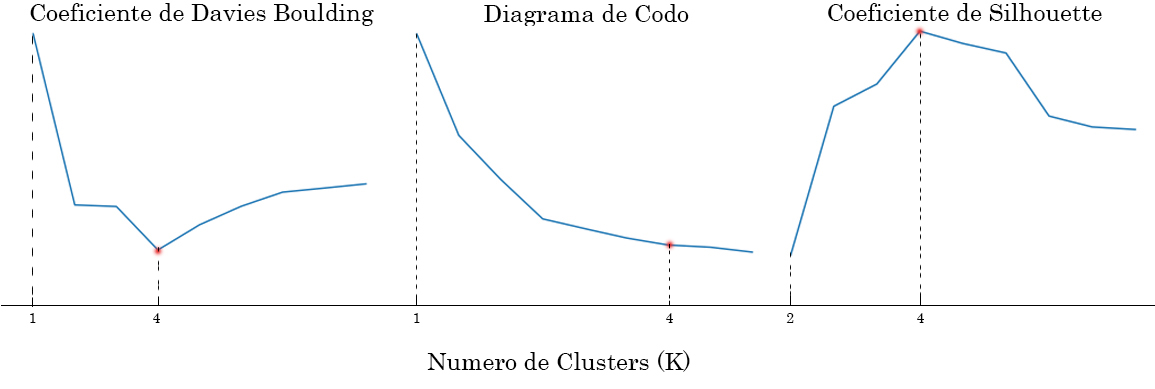
\includegraphics[width=0.8\textwidth]{images/chapter_2/ap_nosup_diagramas}
	\caption{Coeficientes}
	\label{fig:coeficientes}
\end{figure}


\begin{figure}[!h]
	\centering
	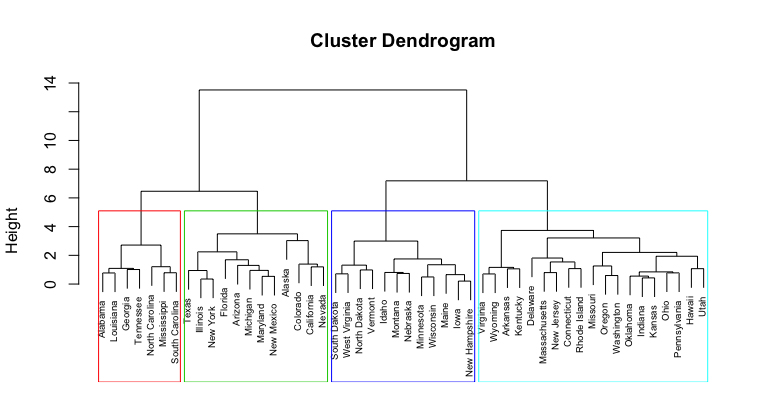
\includegraphics[width=0.8\textwidth]{images/chapter_2/dendograma}
	\caption{Dendograma}
	\label{fig:dendograma}
\end{figure}

\vspace{0.1cm}

% TODO CAMBIAR IMAGEN
\begin{figure}[!h]
	\centering
	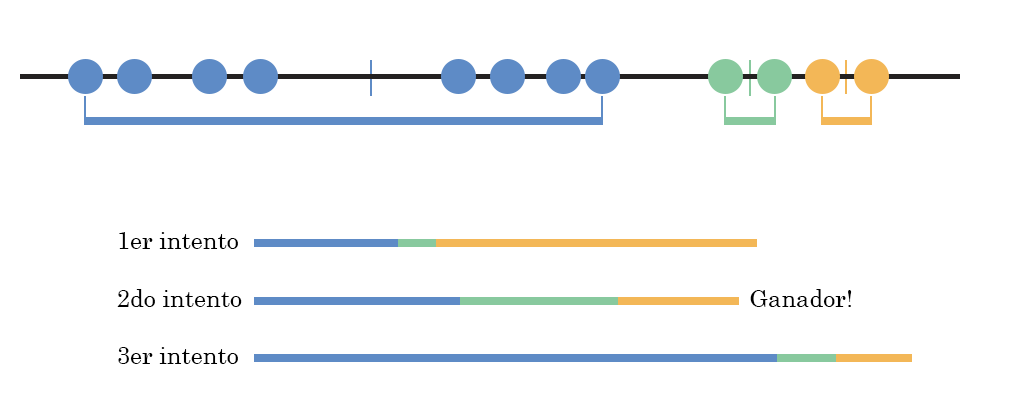
\includegraphics[width=0.7\textwidth]{images/chapter_2/kmedias}
	\caption{KMedias - Busqueda}
	\label{fig:kmediasBusqueda}
\end{figure}


\section{Aprendizaje Supervisado}
Al contrario que el apartado anterior, este tipo de aprendizaje automático, es entrenado con un dataset categorizado con su salida correcta. El algoritmo aprende de este conjunto, para hacer predicciones sobre unos datos desconocidos.

El objetivo de este algoritmo es aprender la función que mapea las variables de entrada en las categorías correctas de salida. Ajusta los parámetros con técnicas de optimización iterativas para minimizar el error en sus predicciones.

Los ejemplos más comunes son la clasificación, para dividir la población en categorías según unos parámetros. Y regresión, que encuentra las correlaciones entre las variables dependientes e independientes.\\

\noindent\textbf{K-Vecinos más Cercanos - KNN}

Simple pero potente, es muy efectivo para tareas de clasificación y regresión. Se basa en la idea de que los puntos de datos similares tienden a agruparse en el espacio de características. Pertenece al paradigma de aprendizaje perezoso o basado en instancias.

\begin{itemize}
	\item Perezoso: no calcula ningún modelo y demora todos los cálculos hasta el momento en que se le presenta un ejemplo nuevo.
	
	\item Basado en instancias: usa todos los individuos disponibles y ante un ejemplo nuevo recupera los más relevantes para componer la solución.	
\end{itemize}

No hay una forma de determinar el mejor valor para K, hay que probar con varias ejecuciones. Valores pequeños de K crea sonido y valores grandes con pocos datos hará que siempre sea la misma categoría. Un valor diferente de K puede cambiar la categoría de un individuo. Figura \ref{fig:knn}

\begin{algorithm}
	\caption{KNN}
	\KwData{poblacion, etiquetas, poblacionPred}
	\KwResult{agrupacion // Clusters para cada individuo de la población}
	agrupacion := $\emptyset$\\
	\For{each individuo $ind$ in $poblacionPred$}{
		// Recorrer toda la poblacion categorizada hasta el momento y clasificar \textit{ind} con los K individuos más cercanos.\\
		agrupacion.append(cluster);
	}
	\Return $agrupacion$\;
\end{algorithm}

La distancia entre individuos más usada es la Euclídea, pero demora más tiempo al aplicar potencias y raíces cuadradas en su cálculo. La distancia Manhattan es más rápida.\\


\noindent\textbf{Redes Neuronales}

Modelo computacional inspirado en el funcionamiento y estructura de las neuronas del cerebro humano. Consiste en capas de nodos interconectados, llamadas neuronas artificiales. Estructura del modelo (Figura \ref{fig:redneu}):


\begin{itemize}
	\item Capa de entrada, en la cual, habrá tantas neuronas como variables de entrada tenga el modelo de predicción.\\
	\item Capa oculta, representada con una o más capas internas. Cada una con su número de neuronas.\\	
	\item Capa de salida, como en la entrada. Tendrá un número de neuronas relacionadas con las variables de salida.
\end{itemize}

Se ha demostrado que tiene un rendimiento notable en muchas tareas, como el reconocimiento de imágenes o procesamiento de lenguaje natural. Aprenden patrones complejos al someterse a un entrenamiento específico con un amplio dataset categorizado.	

En el proceso de entrenamiento aprende a realizar una tarea específica ajustando los parámetros internos (pesos en las conexiones), gracias al dataset proporcionado. Normalmente ajustando con algoritmos de optimización como descenso de gradiente, donde se comparan las predicciones del modelo con las categoría correcta, y actualizando los parámetros del modelo con un método de propagación hacia atrás, backpropagation en inglés. Estos valores se actualizan dependiendo del error cometido y la tasa de aprendizaje proporcionada al modelo.



\begin{algorithm}
	\caption{Red Neuronal}
	\KwData{entrenamiento, etiquetas, evaluacion // Individuos sin categorizar\\
			\Indp \Indp repeticiones, capas // Tam. entrada, oculta, salida}
	\KwResult{pesos // Opcionalmente, devolver los pesos de la red}
	pesos := init(); // Inicializar los pesos de manera aleatoria\\
	\For{$rep \leftarrow 0$ \KwTo $repeticiones$}{
		\For{each individuo $ind$ in $entrenamiento$}{
			// Suma el valor recibido de la capa anterior multiplicada por los pesos de la capa actual con la siguiente. Así se determina la importancia de conexión entre las neuronas. \\
			// Con el valor calculado se aplica a una función de activación y se pasa a la siguiente capa hasta llegar a la salida.\\			
			\textbf{forward();}\\
			// El valor predicho calculado en la salida es comparado con la etiqueta, y se calcula el error. Este error se manda para atrás actualizando los pesos. Se suma la multiplicación del valor predicho en cada capa con la tasa de aprendizaje y el error.\\			
			\textbf{backpropagation();}
		}
	}
	
	
	\Return $agrupacion$\;
\end{algorithm}

%\vspace{0.2cm}

\begin{figure}[!h]
	\centering
	
	
	\begin{subfigure}[t]{0.33\textwidth}
		\centering
		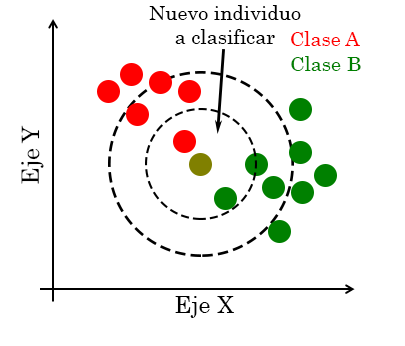
\includegraphics[width=\textwidth]{images/chapter_2/knn}
		\caption{KNN}
		\label{fig:knn}
	\end{subfigure}
	\hfill
	\begin{subfigure}[t]{0.48\textwidth}
		\centering
		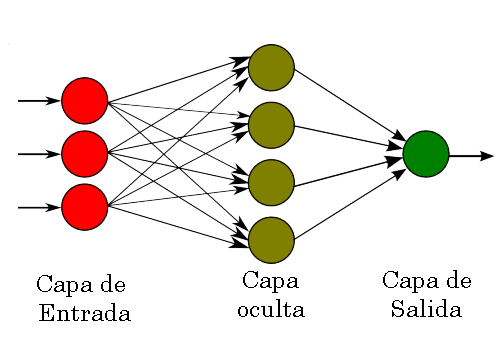
\includegraphics[width=\textwidth]{images/chapter_2/redneu}
		\caption{Red Neuronal}
		\label{fig:redneu}
	\end{subfigure}
	
	\caption{Aprendizaje Supervisado}
	\label{fig:aprendizajeSupervisado}
\end{figure}

\newpage









\section{Programación Evolutiva}


La programación evolutiva es una técnica de optimización inspirada en la teoría de la evolución biológica. Se basa en el concepto de selección natural y evolución de las poblaciones para encontrar soluciones a problemas complejos. 

La población está compuesta por individuos, que pueden ser representados con arrays de números reales, binarios o un árbol, en programación genética. Los individuos tienen un cromosoma, que a su vez tiene uno o varios genes, con uno o más alelos. Esta población es sometida a métodos de selección, mutación y evaluación, para, con el paso de las generaciones maximizar o minimizar un valor fitness.

Esta técnica es muy útil para problemas de optimización donde los métodos tradicionales son bastante lentos.  Se han aplicado a varios dominios, como por ejemplo la bioinformática o robótica \cite{contreras2015mobile}.


\begin{figure}[!h]
	\centering
	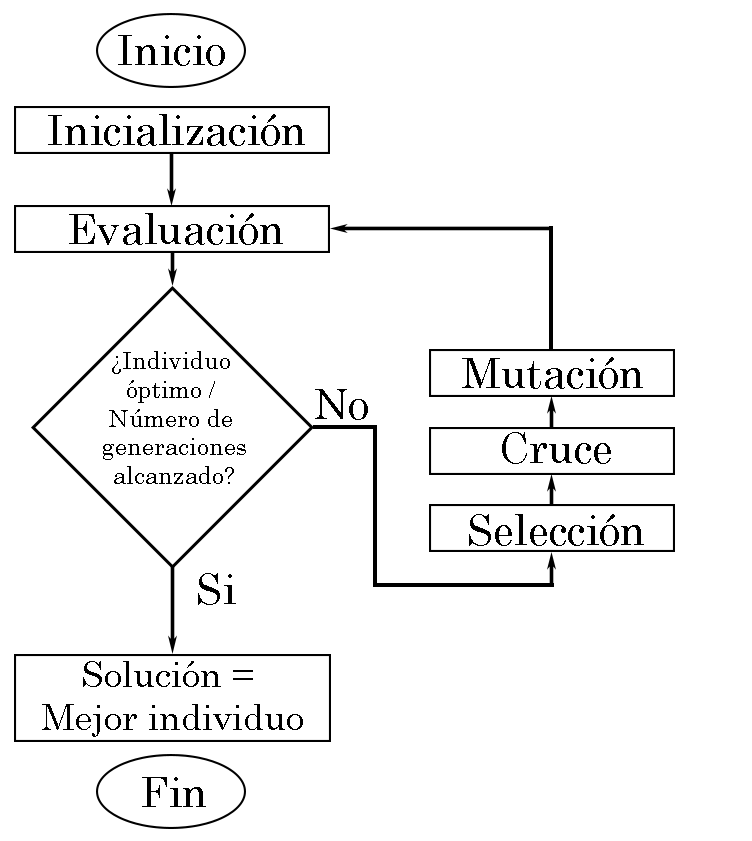
\includegraphics[width=0.4\textwidth]{images/chapter_2/AG}
	\caption{Algoritmo Evolutivo}
	\label{fig:AG}
\end{figure}


\newpage

























%Aquí comienza la descripción del trabajo realizado. Se deben incluir tantos capítulos como sea necesario para describir de la manera más completa posible el trabajo que se ha llevado a cabo. Como muestra la figura \ref{fig:sampleImage}, está todo por hacer.
%
%\begin{figure}[h]
%	\centering
%	\includegraphics[width = 0.5\textwidth]{Imagenes/Vectorial/Todo.pdf}
%	\caption{Ejemplo de imagen}
%	\label{fig:sampleImage}
%\end{figure}
%
%Si te sirve de utilidad,  puedes incluir tablas para mostrar resultados, tal como se ve en la tabla \ref{tab:sampleTable}.
%
%
%\begin{table}
%	\centering
%	\begin{tabular}{c|c|c}
%		\textbf{Col 1} & \textbf{Col 2} & \textbf{Col 3} \\
%		\hline\hline
%		3 & 3.01 & 3.50\\
%		6 & 2.12 & 4.40\\
%		1 & 3.79 & 5.00\\
%		2 & 4.88 & 5.30\\
%		4 & 3.50 & 2.90\\
%		5 & 7.40 & 4.70\\
%		\hline
%	\end{tabular}
%	\caption{Tabla de ejemplo}
%	\label{tab:sampleTable}
%\end{table}
